\chapter{Umsetzung}
\label{cha:Umsetzung}

\section{Hadoop}
\label{sec:Hadoop}

\subsection{HDFS}
\label{hdfs}

Das HDFS ist Bestandteil des Hadoop Frameworks und erfüllt folgende Anforderungen:

\begin{itemize}
\item Betrieb auf Commodity-Hardware
\item Ausfallsicherheit einzelner Knoten
\item Speicherung und Verarbeitung großer Datenmengen
\item Einfache Skalierbarkeit
\end{itemize}

Ein einziger Masterknoten, genannt Name-Node, verwaltet alle Metadaten des Dateisystems, darunter Verzeichnisstrukturen, Dateien und Dateizugriffe der Clients (Apache Software Foundation, 2013). Parallel dazu existieren mehrere Data-Nodes, die den Speicher verwalten, der den entsprechenden Knoten im Cluster zugeordnet ist. Das HDFS bietet ein Set an Funktionen an, das es erlaubt, Daten in das Dateisystem zu schreiben und daraus zu lesen. Es ist nicht nötig, eine eigene Partition für ein HDFS anzulegen, denn es setzt auf einem existierenden Dateisystem, z.B. dem gängigen ext4 (Fourth Extended Filesystem), auf.

\pagebreak

\subsection{Einrichtung und Konfiguration}
\label{subsec:einrichtungkonfig}

Bei der Installation von Hadoop unterscheidet man hauptsächlich zwischen drei möglichen Konfigurationsarten:

\begin{figure}[!htb]
	\centering
	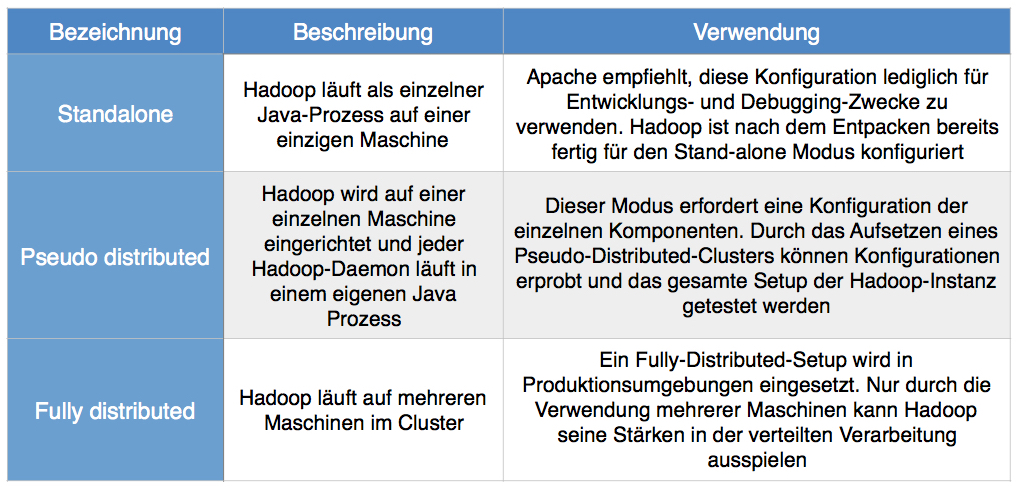
\includegraphics[width=0.9\textwidth]{hadoopconfigtypes}
	\caption{Hadoop Konfigurationsarten}
	\label{img:hadoopconfigtypes}
\end{figure}

Für unseren Use-Case ist die pseudo distributed Variante die Lösung, die unseren Anforderungen am besten entspricht. Mit dieser Konfiguration lassen sich die Funktionalitäten von Hadoop in einem virtuellen Cluster vollständig umsetzen. Hadoop wird offiziell von der Apache Software Foundation\footnote{Apache Software Foundation: http://hadoop.apache.org/releases.html} für Unix-Systeme zur Verfügung gestellt.


Um das Hadoop Framework auf einem Unix-System zu installieren, muss Java, sowie SSH installiert sein.

Anschließend müssen die Konfigurationsdateien von Hadoop angepasst werden, um die gewünschte Konfiguration umzusetzen. Dabei ist eine Anpassung der folgenden Konfigurationsdateien erforderlich:

\textbf{core-site.xml}

\lstset{language=XML}

\begin{lstlisting}
<configuration>
      <property>
          <name>fs.defaultFS</name>
          <value>hdfs://hadoop:9000</value>
      </property>
 </configuration>
\end{lstlisting}

\textit{fs.defaultFS} in Zeile 3 bestimmt, wo der \textit{Name-Node} zu finden ist. Der \textit{Name-Node} wird mithilfe eines Pfads angegeben. Dabei gibt der Pfad den Rechner-Knoten an, auf dem das HDFS betrieben wird. In diesem Beispiel läuft das HDFS auf dem Rechner mit dem Hostname \textit{hadoop} und der Service ist über den Port \textit{9000} ansprechbar. 

\pagebreak

\textbf{hdfs-site.xml}

\lstset{language=XML}

\begin{lstlisting}
<configuration>
    <property>
        <name>dfs.replication</name>
        <value>1</value>
    </property>
</configuration>
\end{lstlisting}


Durch die Eigenschaft \textit{dfs.replication} wird festgelegt, wie viele Kopien der zu verarbeitenden Daten später auf dem Cluster verteilt werden sollen. Da in diesem Fall nur ein Knoten verwendet wird, kann man lediglich eine Kopie speichern.

\textbf{mapred-site.xml}

\lstset{language=XML}

\begin{lstlisting}
<configuration>
    <property>
        <name>mapreduce.framework.name</name>
        <value>yarn</value>
    </property>
</configuration>
\end{lstlisting}

In der obigen Datei wird bestimmt, dass das neue Map-Reduce-Framework \textit{YARN} benutzt wird.

\textbf{yarn-site.xml}

\lstset{language=XML}

\begin{lstlisting}
<configuration>
	<property>
		<name>yarn.nodemananger.aux-services</name>
		<value>mapreduce_shuffle</value>
	</property>
	<property>
		<name>yarn.nodemanager.aux-services.mapreduce.shuffle.class</name>
		<value>org.apache.hadoop.mapred.ShuffleHandler</value>
	</property>
	<propery>
		<name>yarn.nodemanager.vmen-pmem-ratio</name>
		<value>3</value>
	</property>
	<property>
		<name>yarn.nodemanager.delete.debug-delay-sec</name>
		<value>600</value>
	</property>
</configuration>
\end{lstlisting}

Die Eigenschaften in den Zeilen 3 und 7, legen fest, wie Hadoop später die Verteilung (Mischung) der Knoten im Cluster handhaben wird. Der \textit{yarn.nodemanager.vmem-pmem-ratio} stellt das Verhältnis von physikalischem zu virtuellem Speicher dar. Verwenden wir beispielsweise 4 GB RAM, stehen im Cluster 4 * 3 = 12 GB virtueller Speicher für die Ausführung der Map-Reduce-Jobs oder YARN-Anwendungen zur Verfügung. Die Eigenschaft in Zeile 15 gibt an, wie viel Sekunden die Anwendungsdaten für auf \textit{YARN} laufende Anwendungen bestehen bleiben, bevor sie automatisch gelöscht werden. 


\pagebreak

\subsection{Web-Interface von Hadoop}
\label{subsec:webinterface}

Sobald die Services von Hadoop konfiguriert und erfolgreich gestartet wurden, kann man über die zur Verfügung stehenden Web-Interfaces den aktuellen Status des Clusters und seiner einzelnen Knoten abfragen. Mithilfe der IP-Adresse und dem zugehörigen Port lassen sich folgende Seiten abrufen:

\textbf{Übersicht von Hadoop und dessen Name-Node über den Port \textit{50070}}
Die Seite gibt Informationen zur installierten Hadoop-Version, zum verfügbaren Festplattenspeicher, zur Startzeit des Clusters, sowie den Status der vorhandenen Knoten.

\textbf{Übersicht der laufenden und abgeschlossenen Jobs auf dem Cluster, über den Port  \textit{8088}}
Die Übersicht zeigt zum Einen den Status einzelner Knoten im Cluster und zum Anderen Anwendungen, die im Cluster ausgeführt werden/wurden. Dabei lassen sich Log Files der absolvierten Jobs anschauen, um eventuelle Fehler ausfindig zu machen.

\subsection{Map-Reduce}
\label{subsec:mapreduce}

Im Jahr 2004 veröffentlichten zwei Google-Mitarbeiter ein Paper (Dean et al., 2004) zu einem neuen Ansatz, um große, unstrukturierte Daten anzuzeigen und darin suchen zu können. Aus dem Problem heraus, dass die im Unternehmen gespeicherten Datenmengen zu schnell und zu stark wuchsen, um sie mit herkömmlichen Mitteln verarbeiten zu können, entstand das in dem Paper vorgestellte Programmiermodell \textit{Map-Reduce}. Es beschreibt nicht nur, wie man große Datenmengen durchsucht, auswertet und in Schlüssel-Wert-Paare zusammenfasst, sondern auch, wie man diese sogenannten Map-Reduce-Jobs effizient über ein Cluster auf \textit{Commodity-Hardware} ausführt. Die Arbeitsweise des Algorithmus lässt sich in drei Prozessschritte unterteilen.

\begin{figure}[!htb]
	\centering
	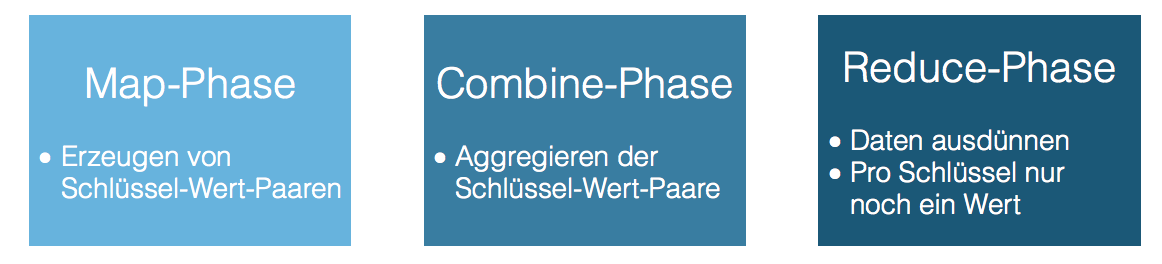
\includegraphics[width=0.9\textwidth]{mapreducephases}
	\caption{Die drei Prozessschritte des Map-Reduce Algorithmus}
	\label{img:mapreducephases}
\end{figure}